%!TEX root = main.tex


\chapter{Introduction}\label{ch:intro}

Program modularity is not a radical idea. From early on, programmers have established from experience that breaking programs apart into smaller more managable pieces is a good idea. Steadily, this idea found its way into the design of programming languages. The ML module system is a powerful language for constructing and abstracting over modules in statically-typed languages. Decomposing a program into modules should not compromise the type-safety guarantees afforded by modern statically-typed languages. The module system itself must have a type system that ensures type-safe composition. 

A module system typically partitions code into interfaces (also called signatures) and implementations. Signatures describe the shape of the implementation by listing values and types exported from modules. Implementations rely on signatures to help typecheck occurrences of imported names. A central question in module system design is what should go into signatures. On the one hand, signatures must provide information to typecheck external module dependencies. On the other, signatures should not contain too much information so as to compel the programmer to recapitulate the implementation of the dependency in the corresponding signature. 

The main subject of this dissertation is the type system and semantics of an intuitive variant of the ML module system, the true higher-order module system (THO). As I will show, this module system is both type-safe and intuitive in that its semantics is based on $\beta$-reduction. 
The implementation of the higher-order module system has evolved considerably since the seminal MacQueen-Tofte paper~\cite{mt94} which was the original description of true higher-order semantics. The goal of the rest of this dissertation is to formalize, simplify, extend, and improve the static semantics of true higher-order module systems. 
%I focus on changes in module representations and improvements in elaboration algorithms. 
This dissertation studies what this true higher-order semantics means precisely and formally by giving a modern formal account. These results open the way to exploration of the design space of \emph{full transparency} (\emph{i.e.}, exactly what can and should propagate through higher-order functor applications) and separate compilation. 
	
\section{Higher-Order Module System}\label{sec:hofct}
	Higher-order modules extend the ML module system with higher-order functors, a natural extension. There are many different applications and three general approaches for higher-order modules~ \cite{tofte92,tofte:jfp94,mt94,biswas95,leroy95,Leroy:generativity,LillibridgeThesis,russothesis,dreyerthesis} which differ mainly on how they handle type sharing in the apply functor (fig.~\ref{fig:applyfctocaml}). 

\lstdefinestyle{ocamlcode}{language=[Objective]Caml}%, numbers=left, numberstyle=\tiny, stepnumber=1, numbersep=5pt}
\begin{figure} 
\begin{lstlisting}[style=ocamlcode]
module type T = sig type t end
module Id = functor(X:T) -> X

module type FS = functor (X:T) -> T

module Apply = functor(X:sig module F : FS module M:T end) -> X.F(X.M)

module M0 = struct type t = unit end	
module M1 = Apply(struct module F=Id module M=M0 end)

let x : M1.t = ();;
\end{lstlisting}
\caption{Apply functor example in OCaml}
\label{fig:applyfctocaml}
\end{figure}
		
In the apply functor example, the higher-order functor Apply applies functor F to a module M. Tofte~\cite{tofte92} introduced the first cut at the semantics for higher-order modules with \emph{non-propagating} functors. Under Tofte's semantics, the apply functor does not propagate the type M0.t through the functor application X.F(X.M), thus M1.t $\ne$ M0.t = unit. It assigns the signature in fig.~\ref{fig:tofteapplysig}. to the apply functor. Notice that the signature for the body does not say anything more about \lstinline{type t}. 
\begin{figure}
\begin{lstlisting}
functor Apply(X: sig functor F : (X: T) : T structure M : T end) : T
\end{lstlisting}
\caption{Signature assigned to Apply functor under MacQueen-Tofte semantics}
\label{fig:tofteapplysig}
\end{figure}

MacQueen-Tofte~\cite{mt94} argues that the type sharing M1.t = M0.t = unit should hold. The strong sums model of modules also predicts this behavior of full type propagation \cite{macqueen:popl86}. The semantics in MacQueen-Tofte, \emph{true higher-order functors} or \emph{fully transparent generative functors}, re-elaborates the functor body of apply given the contents of X.F and X.M at the point of the functor application on line 14. Although this re-elaboration has the desired effect of propagating types, MacQueen-Tofte assigns exactly the same functor signature as the Tofte semantics. Leroy~\cite{leroy95} offered an alternative approach, \emph{applicative functors}, that enriched the notion of type paths in functor signatures with functor applications such as F(M).t. Applicative functor semantics assigns the functor signature in fig.~\ref{fig:appapplysig}. 

\begin{figure}
\begin{lstlisting}
functor Apply(X : sig functor F : FS structure M : T end) :
          sig type t = X.F(X.M).t end
\end{lstlisting}
\caption{Signature assigned to Apply functor under applicative functor semantics}
\label{fig:appapplysig}
\end{figure}

However, applicative functors only solve the type propagation problem under certain circumstances and loses the generative semantics of functors, \ie, functor applications do not generate fresh tycons to enforce abstraction. To address this shortcoming, Moscow ML and Dreyer's module system~\cite{dhc03} combined applicative and non-propagating generative higher-order functors in the same language. Fully transparent generative functors both solve the type propagation problem under all circumstances and do not compromise on generative functor semantics. In the last decade, researchers have gained significant experience in engineering non-fully transparent generative functors and transparent applicative functors in compilers such as Moscow ML and OCaml. Although they differ internally, both SML/NJ and MLton compilers support some variant of true higher-order functors semantics. I take OCaml and SML/NJ as representatives of the former and latter groups respectively.
	 
Under both OCaml and SML/NJ compilers, the apply functor example typechecks. Furthermore, although applicative functors cannot directly handle applications to nonpaths, lambda lifting the offending nonpath generally solves that issue. However, if I modify the apply functor slightly by applying a formal functor F to \lstinline{struct type t = int end} as in fig.~\ref{fig:hoapplyfct}, then applicative functors fail to propagate enough type information. When the typechecker gets to line 3 in fig.~\ref{fig:hoapplyfct}, it does not have enough information about F to give a stronger signature for ApplyToInt's functor body. Neither is there a path to the argument \lstinline{struct type t = int end} used to construct an applicative functor path. Because the typechecker must give the functor body a signature immediately in order to give HO functor ApplyToInt a complete signature, it can only give the weakest signature, \lstinline{sig type t end}. A-normalization gets the program to typecheck but unnecessarily clutters up the code. Thus, in this sense, applicative functors cannot be said to be fully transparent. The SML/NJ compiler has no such restrictions.

\begin{figure}
\hrule
\begin{lstlisting}[style=ocamlcode]
module ApplyToInt = functor (F : functor (X:T) -> T) -> F(struct type t = int end)

module R = ApplyToInt(Id)
let x : R.t = 5;;
\end{lstlisting}

OCaml functor signature for ApplyToInt
\begin{lstlisting}
module ApplyToInt : functor (F : functor (X : T) -> T) -> sig type t end
\end{lstlisting}
OCaml type error:
\begin{verbatim}
This expression has type unit but is here 
used with type R.t = ApplyToInt(Id).t
\end{verbatim}
SML/NJ functor signature for ApplyToInt
\begin{lstlisting}
functor ApplyToInt(functor F : (X: T) : T end) : T

structure R = ApplyToInt(Id)
val x : R.t = 5
\end{lstlisting}
SML/NJ types x as R.t 
\hrule
\caption{OCaml and SML/NJ versions of ApplyToInt functor}
\label{fig:hoapplyfct}
\end{figure}

The example in figs.~\ref{fig:hoapplyfct} illustrates the fundamental problem with applicative functors. A higher-order ApplyToInt functor fails to properly propagate types under Leroy's applicative functor semantics. Consequently, the last line fails to typecheck. They work well as long as the relationship between functor parameter and body is simple, \ie, can be captured in the extended notion of a path with functor application or by A-normalizing the argument. However, not all possible functors fit into this mold. Having to A-normalize arguments of functor applications is an unnecessary shortcoming. Making an argument structure a local definition for the functor application does not help because then after the functor application, the argument structure name would be out of scope. True higher-order functors propagate types across all functor applications with no change to the source. The solution that MacQueen and Tofte \cite{mt94} advocate is a re-elaboration of the functor body given the actual argument module.

 \begin{figure}
\begin{center}
 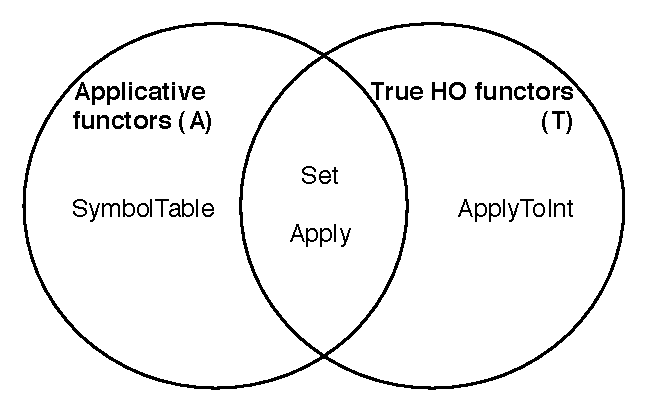
\includegraphics[scale=0.5]{../design/figs/appandtruetypeprogvenn.pdf}
\end{center}
 \caption{Examples of applicative functors and true higher-order functors}
 \label{fig:appandtruetypeprogvenn}
 \end{figure}

% Show example. explanation of related work should be self-contained "mini-essays"
In instances such as the SymbolTable functor (fig.~\ref{fig:symtbl}), applicative functors admit too much sharing as noted by Dreyer \cite{dreyerthesis}. Applicative functors would permit the symbols from one SymbolTable ST1 to be used to index another ST2 despite the sealing of the functor body to signature SYMBOL\_TABLE. Both OCaml and SML/NJ elaborators will make the symbol type abstract, but in OCaml it is only abstract with respect to external clients and not other instances of SymbolTable. Because SymbolTable is applied to the same empty argument for both ST1 and ST2, the two instances also share the same symbol type according to applicative functor semantics. This behavior breaks an important abstraction. Generative functors are more appropriate for enforcing the exact kind of abstraction desired. In contrast, applicative functor semantics are appropriate for some purposes such as the Set functor in fig.~\ref{fig:setfct} where the type sharing of Item.item is desirable and it is acceptable to use items in Sets of the same type interchangeably. However, it is debatable whether the Set functor is a common case. The set of programs T for which true higher-order functors propagate types is exactly those one would want to propagate types. T partially overlaps with the set A the programs such that applicative functor semantics propagates types. In contrast, one should not propagate types in the set $A\\T$. Dreyer~\cite{dreyerthesis} noted correctly that applicative functors and non-fully transparent generative functors are incomparable. Neither applicative nor true higher-order functors can subsume the other. However, there remains the pragmatic question whether the programs that propagate types under applicative functors but not under true higher-order functors ought to have propagated the types in those cases. 

\begin{figure}
\hrule
~
\begin{center}
\begin{tabular}{c}
\begin{lstlisting}
signature SYMBOL_TABLE = 
sig 
  type symbol 
  val string2symbol : string -> symbol 
  val symbol2string : symbol -> string 
  ... 
end 

functor SymbolTable () = 
struct 
  type symbol = int 
  val table : HashTable.t = HashTable.create (initial size, NONE) 
		(* allocate internal hash table *)		
  fun string2symbol x = 
		(* lookup (or insert) x *) ... 
  fun symbol2string n = 
	(case HashTable.lookup (table, n) of 
		  SOME x => x 
		| NONE => raise (Fail "bad symbol")) 
    ... 
end :> SYMBOL_TABLE 

structure ST1 = SymbolTable() 
structure ST2 = SymbolTable() 
\end{lstlisting}
\end{tabular}
\end{center}
\hrule
\caption{SymbolTable functor example from Dreyer~\cite{dreyerthesis}}
\label{fig:symtbl}	
\end{figure}

\begin{figure}
\hrule
~
\begin{center}
\begin{tabular}{c}
\begin{lstlisting}
signature COMPARABLE = 
sig 
  type item 
  val compare : item * item -> order 
end 
functor Set (Item : COMPARABLE) = 
struct 
  type set = Item.item list 
  val emptyset : set = [] 
  fun insert (x : Item.item, S : set) : set = x::S 
  fun member (x : Item.item, S : set) : bool = ... Item.compare(x,y) ... 
  ... 
end 
\end{lstlisting}
\end{tabular}
\end{center}	
\hrule
\caption{Set functor example from Dreyer~\cite{dreyerthesis}}
\label{fig:setfct}
\end{figure}

The original criticisms of the MacQueen-Tofte semantics are that it lacks
support for true separate compilation and that the stamp-based
operational semantics makes it difficult to extend the module system
and to reason about it. Many recent treatments of ML module systems
abandon true higher-order functors completely due to these
issues. The claim is that the type-theoretic presentations of the
module system with applicative functors address these problems. This
dissertation will consider the question whether an operational
semantics account must necessarily be more complicated and if so,
why. In contrast to recent work, this dissertation will take true
higher-order module behavior as the starting point for developing a formal semantics while addressing these criticisms and concerns. My formalism follows behavior of the SML/NJ compiler which enriches the internal representation of functors and functor signatures to express the static actions of the functor, thus avoiding a re-elaboration of the functor body. This approach will also yield some practical benefits. The SML/NJ and MLton implementations have not kept up with the pace of the progress in module system design at least partially due to the fact that most of the research has been a radical departure from true higher-order module semantics. Reframing the state-of-the-art in terms of true higher-order module semantics will bring recent developments closer a practical extension in these production-quality compilers. 

\section{Full Transparency and True Separate Compilation}
		Since MacQueen and Tofte introduced true higher-order modules, many researchers~\cite{leroy94,russothesis,mixml} have studied how to downgrade higher-order functors to regain true separate compilation, \ie, Modula-2-style separate compilation. To workaround this limitation, SML/NJ \cite{am:pldi94,hlpr:tr94} uses a powerful compilation manager CM \cite{blume95:cm}, which uses a pickled static environments that include complete static descriptions going beyond syntactic signatures. However, using a pickled static environment does not solve the true separate compilation problem. 
		
		The separate compilation problem can be reframed as a completeness problem for the signature language, \ie, can the source-level signature language adequately describe all possible modules including functors. Currently, the SML/NJ compiler elaborates module syntax into internal semantic objects. These semantic objects are expressive enough to encode the functor body relationships that eluded the source signature language. The source and these semantic objects are then compiled to a predicative System F$_\omega$-like calculus \cite{shao98}. This suggests that an F$_\omega$-like calculus should be expressive enough to characterize all the static semantic actions of functors. In chapter~\ref{ch:entitycalc}, I describe the entity calculus, a small language that precisely complements the signature calculus and fully describes module types. The semantics is a foundation for future work on the question of separate compilation in higher-order module systems. 
		
		Intuitively, true higher-order modules cannot be fully expressed in the syntactic signature language because it is limited to definitional specs and type sharing. For example, there is no way to express a functor signature for the apply functor that accounts for all sharing due to full transparency. Therefore true higher-order modules cannot in general be separately compiled. In particular, HO functor applications cannot always be separately compiled from the functor definition. In the past, various researchers have approached this problem by incorporating applicative functors into the language to varying degrees \cite{leroy95,biswas95,russothesis,dhc03} sometimes limiting the generative functors in the process. In this dissertation, I will argue that applicative functors cannot replace true higher-order functors in the general case. Moreover, if fully transparent generativity is the goal, then applicative functors only serve to support true separate compilation in a limited number of cases. 
		
		% In order to have true separate compilation, the surface signature language must be able to express the full signature of all structures and functors. Even in a module language that only supports first-order functors, this requirement proves to be a problem because the signature language is be unable to express generative types in the body of a functor. Generative types in the body of a functor do not have externally expressible names prior to functor application. 
		
		
% \subsection{Signature calculus}
% 	Since the study of the true separate compilation problem points in the direction of the signature calculus, it will be fruitful to take this opportunity to reconsider the design of ML's signature language. After Harper-Lillibridge and Leroy, despite the continuing pace of the development of ML module systems, the signature language generally did not see much attention except for Ramsey \etal's paper\cite{ramsey05}. Ramsey \etal~\cite{ramsey05} describe a signature language that includes operations for post hoc manipulation such as adding, removing, rebinding components, and merging signatures. SML/NJ's semantics for \lstinline{include} is richer than the simple syntactic inclusion found in the Definition\cite{mthm97}. In particular, certain kinds of compatible signatures can be merged. In the SML/NJ 110.68 compiler, two signatures are {\bf compatible} when their overlapping specifications (\ie, specifications with the same name) have the same arity and follow the rules summarized in table~\ref{tbl:njsigmerge}. However, the current compatibility rules are inconsistent and incomplete. For example, merging an eqtype and a type specification results in an eqtype in one direction and a type in the other as shown in fig.~\ref{fig:compatmerge}. 

% \begin{figure}
% \begin{lstlisting}
% signature S0 = sig eqtype t end
% signature S1 = sig type t end
% signature S2 = sig include S0 include S2 end 

% S2 : sig eqtype t end

% signature S0 = sig type t end
% signature S1 = sig eqtype t end
% signature S2 = sig include S0 include S2 end

% S2 : sig type t end	
% \end{lstlisting}
% \caption{Unsound behavior of SML/NJ signature merging by \lstinline{include}}
% \label{fig:compatmerge}
% \end{figure}
	
% Despite its present incomplete state, SML/NJ can do the appropriate consistent merge for Garcia \etal's example (fig.~\ref{fig:garciasigmerge}). In the case of Garcia \etal's example, the typechecker needed to do is to note that the repeated components $t$ and $u$ due to inclusion are identical specifications. 
	
% 	The SML/NJ semantics goes further and merges consistent yet unequal specifications such as abstract types and datatypes. The merging semantics can be substantially improved by making the table more symmetrical and adjusting some of the precedences to something more sensible. Both Ramsey \cite{ramsey05} and Dreyer and Rossberg \cite{mixml} offer language support for a signature calculus that can safely compose signatures, effectively permitting a kind of multiple signature inheritance. Both accounts only model signature merging for a small language without support to features such as eqtype and generative datatypes. In particular, a fine-grain merging of eqtype can be nontrivial. For example, it is safe to merge \lstinline{eqtype t} and \lstinline{datatype t = K} where K is a data constructor. In contrast, merging \lstinline{eqtype t} and \lstinline{datatype t = K of int -> int} is unsafe. Consistent merge rules of this flavor can already be found elsewhere in the compiler, namely in signature matching. This dissertation will develop a formal semantics for a safe but flexible consistent signature merging that covers these features of ML. 

% 				\begin{table}
% 				\begin{tabular}{|l|l|l|l|l|}
% 				\hline
% 				     & type & eqtype & datatype & deftype\\
% 				\hline 
% 				type & \chk & eqtype & \ex & \ex\\
% 				\hline
% 				eqtype & type & \chk & \ex & \ex\\
% 				\hline
% 				datatype & \chk & datatype & \ex & \ex\\
% 				\hline
% 				deftype & \ex & \ex & \ex & \ex\\
% 				\hline
% 				datatype withtype & \chk & datatype withtype & \ex & \ex\\	
% 				\hline
% 				\end{tabular} 
% 				\caption{SML/NJ 110.68 Signature elaboration consistent signature merging: \chk~can be merged, \ex~cannot be merged, otherwise indicates specs mergable but indicated spec takes precedence}
% 				\label{tbl:njsigmerge}
% 				\end{table}
				
% \begin{figure}[ht]
% \hrulefill\\
% \begin{minipage}[b]{0.5\linewidth}
% \begin{lstlisting}[frame=none]
% signature S0 = 
%   sig 
%     type t
%     eqtype u
%   end
% \end{lstlisting}
% \end{minipage}
% \hspace{0.1em}
% \begin{minipage}[b]{0.5\linewidth}
% \begin{lstlisting}[frame=none]
% signature S1 = 
%   sig 
%     include S0
%     val x : int
%   end
% \end{lstlisting}
% \end{minipage}\\
% \begin{minipage}[b]{0.5\linewidth}
% \begin{lstlisting}[frame=none]
% signature S2 = 
%   sig 
%     include S0 
%     val y : unit 
%   end
% \end{lstlisting}
% \end{minipage}
% \hspace{0.1em}
% \begin{minipage}[b]{0.5\linewidth}
% \begin{lstlisting}[frame=none]
% signature S3 = 
%   sig 
%     include S1 
%     include S2 
%   end
% \end{lstlisting}
% \end{minipage}
% \hrulefill
% \caption{The naive macro expansion semantics of the Definition rejects S3. SML/NJ accepts it. This example was derived from Garcia \etal's GraphSig, IncidenceGraphSig, and VertexListGraphSig\cite{garcia05:extendedcomparing05}.}
% \label{fig:garciasigmerge}
% \end{figure}

% The signature merging semantics found in Ramsey \etal~is quite aggressive. In one example (fig.~\ref{fig:ramseymerge}), the merging semantics creates a new definitional type spec \lstinline{type u = t} in order to merge two signatures that disagree on an entangled value specification \lstinline{val x : t list} and \lstinline{val x : u list}. This kind of aggressiveness likely goes beyond the intention or expectation of the programmer. The programmer may have difficulty deciphering typechecking errors relating to S2.u and S2.x after this point because of this aggressive induced type sharing. It would be more sensible to have the typechecker complain that S0.x and S1.x are incompatible value specifications because as far as the typechecker and programmer are concerned, S0.t and S1.u are simply flexible type specifications. 

% \begin{figure}[ht]
% \hrulefill\\
% \begin{minipage}[b]{0.5\linewidth}
% \begin{lstlisting}[frame=none]
% signature S0 =
% sig
%   type t
%   type u 
%   val x : t list
% end
% \end{lstlisting}
% \end{minipage}
% \hspace{0.1cm}
% \begin{minipage}[b]{0.5\linewidth}
% \begin{lstlisting}[frame=none]
% signature S1 = 
% sig
%   type t
%   type u 
%   val x : u list
% end	
% \end{lstlisting}	
% \end{minipage}\\
% \begin{lstlisting}[frame=none]
% signature S2 =
% sig
%   type t 
%   type u = t
%   val x : t list
% end	
% \end{lstlisting}
% \hrulefill
% \caption{This is an example from Ramsey \etal \cite{ramsey05}. S2 is the merge (greatest lower bound) of S0 and S1 according to their semantics.}
% \label{fig:ramseymerge}
% \end{figure}

% Inspired by Ramsey \etal, my study of signature calculi will go beyond the semantics of consistent signature merging to consider the design implications of adding parameterized signatures\cite{jones96}, signature variables, and related features to the ML signature language.
% The ML signature language permits type definitions that may refer to general type expressions. Type expressions may involve both primitive type constructors such as $\rightarrow$ and programmer-defined type operators. It is the inclusion of type operators that gives the signature language much of its expressiveness. The semantics of type sharing constraints differs significantly between SML90 and SML97. Type sharing constraints could be imposed on two type constructors without restriction in SML90. In SML97, the designers partitioned the semantics of type sharing into type definitions which expressed sharing between an abstract type and an arbitrary type expression, and regular type sharing constraints which can only be imposed between two flexible (or primary) types whose names must be in scope. 

% 				A module system that permits both type definitions and type sharing constraints in signatures introduces significant new complexity. For example, whereas in Leroy's \cite{Leroy:generativity} TypModl language, which only permits SML90-style definitional type sharing constraints and no type definitions, type sharing constraints can be ``normalized'' by pushing them up the signature and eliminated by turning them into type definitions, type sharing constraints cannot be eliminated in a language that permits both type definitions and type sharing constraints. 

% In ML modules, structures can be arranged in a hierarchy. This feature enables flexible namespace management. In contrast, signatures cannot be arranged in such a hierarchy. Signatures must be defined at the top-level and can never be enclosed in any other signature or module. For complex hierarchies such the SML/NJ's Control module that contains layers of submodules, the corresponding signature CONTROL and the signatures of the submodules PRINT and ELAB are related only incidentally by occurrence in structure specifications in CONTROL. This shortcoming in the signature language unnecessarily pollutes the signature namespace and complicates browsing through and working with highly nested hierarchies. It would be desirable to permit (transparent) signature specifications within signatures. For added flexibility and perhaps increased expressiveness, it may be useful permit signature definitions within structures and functors. Furthermore, in order for modules to match these signatures enriched with signature specifications, modules must permit corresponding signature definitions. 

% \begin{figure}
% \begin{lstlisting}
% structure M = 
%   struct 
%     type t = int 
%     type u = bool * string 
%     val a : u * t
%   end 
% signature S = sign(M) removing u adding val b : t * t	
% \end{lstlisting}	
% \caption{Accessing and modifying (via Ramsey \etal~signature operations) an inferred signature}
% \label{fig:inferred}
% \end{figure}

% Since the semantics of ML already supports the extraction or inference of module signatures from the implementation, perhaps it makes sense to permit the programmer to operate directly on the inferred signatures of implementations (modules) or generate/synchronize module implementation based on the signature. Programmers often skip the step of writing proper signatures for modules because the necessary notation is cumbersome and potentially repetitive with respect to the module implementations of signatures. Some programming environments can help programmers automatically generate interfaces, but changes usually are not propagated bidirectionally. Synchronization of modules and signatures is ill-defined in the ML module system which supports a many-to-many relationship between modules and signatures. However, this is exactly where the existence of a principal signature or of a full signature might be useful. If programmers can leverage the structure of existing module structure when writing signatures, this might lower the barrier of entry for programmers with existing non-modularized source thus providing a path to ``gradual modularization''. For example, in fig.~\ref{fig:inferred} an inferred signature can be modified after the fact to serve as a template for future structures without having to explicitly write out any signature. This signature language will enable programmers to quickly integrate modular and non-modular code by facilitating rapid construction of variations on inferred signatures. Admittedly, this feature may run against the very spirit of splitting out explicit interfaces from implementations. 

% \section{Secondary Research Problems}
% \subsection{Static effects} including generative v. MixML mutation of types 
% \subsection{Module linking} functional and ad hoc linkage to show MixML is a radical departure from ML computational linking (the computation that happens before linking to produce the environments/closures that go along with the functions to be linked)

%% \section{Principal Goals of Research} Maybe here???
% \subsection{Polymorphism}
% \subsection{Generativity and abstraction}

				
% \section{Methodology}
% 	Informed by MixML, MacQueen-Tofte semantics, and FLINT semantics as the main sources of inspiration, my dissertation research will define a new formal semantics (including a dynamic semantics) and type system for true higher-order module system based on the current module system design in the SML/NJ compiler. The semantics will clarify and extend the implicit compiler semantics. Part of this study will include experimental prototypes evaluated according to the design criteria outlined above. This prototype module system will validate the practicality of the formal design. The prototype will include a module language elaborator including typechecker and basic compilation into a suitable typed intermediate language. 
	
% 	Through the course of formalizing the module system, the dissertation will establish type soundness of the module language for the dynamic semantics and type system in the style of Owens-Flatt but for the more powerful ML module system. Moreover, it will precisely define full transparency, separate compilation, and the relationship between the two. The hypothesis is that these two features are mutually exclusive because I conjecture that typechecking a signature language powerful enough to encode all possible relationships between functor parameter and body would be undecidable. If the hypothesis turns out to be false, then the dissertation should develop a signature calculus powerful enough to represent all possible static semantic actions of higher-order functor application. The final component of the dissertation will be the decidability and soundness of the signature calculus typechecking. 

\section{Organization}

Chapter~\ref{ch:background} gives an overview of the evolution of module systems and a discussion of related work including some of the latest variants of the ML module system. Chapter~\ref{ch:designspace} outlines and explores the design space of ML module systems. The focus is on the variants of higher-order functor semantics including applicative functors, type generativity, first- and second-class modules, separate compilation, and signature calculus design. It discusses the implications of true higher-order semantics with respect to the other major features of the module system and compares the design with other approaches to higher-order functors  and considers the implication of true higher-order semantics in light of the goal of separate compilation.  

Chapter~\ref{ch:typesystem} introduces the type system for the surface language. The type system is a first-order calculus supporting type constructors. The chapter covers the kind system and static semantics of the type systems. Chapter~\ref{ch:surfacelang} defines the core and module surface (\emph{i.e.}, syntactic) languages. The discussion covers important classifications of type constructors in the context of the module language. 

Chapter~\ref{ch:entitycalc} discusses the entity calculus, a small functional language that precisely defines the functor actions needed to fully express true higher-order semantics. The chapter gives a evaluation semantics for the entity calculus and establishes some key properties along with the semantics for the relativized type languages. The next part of the dissertation formally defines the semantics of the module system in two interweaving modes. Chapter~\ref{ch:homods} introduces the elaboration semantics that both constructs entity calculus expressions and typechecks programs using the result of the evaluation of those expressions. 

Chapter~\ref{ch:translation} defines a system that translates module syntax to an enriched variant of System F$_\omega$ and establishes the soundness of the elaboration semantics based on the soundness of System F$_\omega$'s type system. 

Chapter~\ref{ch:conclusion} outlines some directions for future work and concludes. Appendices~\ref{ch:smlnjsem} and~\ref{ch:impl} discuss semantics and implementation of higher-order modules in SML/NJ and contrasts it with that of the present work. Appendix~\ref{ch:proofs} provides the proofs of the formal properties in above chapters. Finally, Appendix~\ref{ch:notation-index} contains an index of the technical notations used in the body of the dissertation.



% Elsa Gunter, Faninguin (Mike Gordon's student) tried to develop a formal metatheory of Definition ML
% Peripheral goal of formalizing in 
% \section{Applications}
% \subsection{Type functionals vs. applicative functors}
% \subsection{Implied associative types}
% \subsection{Effects}

%%% Local Variables: 
%%% mode: latex
%%% TeX-master: "main"
%%% End: 
